\chapter{Custom EIT Meshes}
\label{chap:chapter-5}

\emph{This work has been presented in part at: 
 the 21st International Conference on Biomedical 
 Applications of Electrical Impedance Tomography (EIT 2021)~\parencite{stowe_generating_2021}.} 

\section*{Acknowledgement}
\emph{Tidal Medical funded the work presented in this chapter.}

\section{Introduction}


\subsection{Background}
\subsubsection{ARDS}
\subsubsection{EIT for ARDS monitoring}
\subsubsection{Custom mesh generation}
\subsection{Motivation}

limitation  of meshing - briwef(1 par sum )

With EIT it is suggested that more accurate models make a more accurate image\dots
The more closely 

\section{Methods}

\subsection{Segment editor}
\subsubsection{Automatic segmentation of the thorax}
\begin{algorithm}[H]
	\SetAlgoLined
	\KwIn{image}
	\KwOut{external boundary}
		weiner filter\;
		Set the lung intensity to 0\;
		erode image using disk size 20\;
		reconstruct on image from line 4\;
		dilate with disk of size 20\;
		reconstruct on image from line 6\;
		binarize, thresh = 0.5\;
		fill holes\;
		close - disk of size 2\;
		open using disk size 5\;
		external boundary = largest object\;
	\caption{Segment the external body boundary.}
\end{algorithm}

\subsubsection{Manual Segmentation Correction}

\subsection{Mesh Generation}
\subsubsection{Extruded Geomerty}
\subsubsection{3D Lung Regions}

\subsection{Evaluation on ARDS patients}

\section{Results}
Data from 4 ARDS patients with CT
and EIT were used to develop a segmentation 
and correction tool to identify 
the lungs and boundary of the body.  
Segmentation was done using the 4th intercostal space, 
with 10 adjacent CT 
slices to form an enclosed chest cavity. 
The lungs
and exterior boundary were identified by increasing the contrast
and identifying an appropriate threshold.
Each segmentation was downsampled to
20 points that could be edited by the user in Matlab. The 
mesh was generated using 
\verb!ng_mk_extruded_model!~\cite{Grychtol2012} in EIDORS 
3.10~\cite{Adler2019}. Images were reconstructed 
using GREIT~\cite{Adler2009}. 
The GI index was calculated using the method
presented by Zhao et al.~\cite{Zhao2009} using the lung regions from the 
forward model. A ventilated lung estimate was made using the
segmentation with equation \fref{eq:ventilated_lung_est}.
\begin{equation}\label{eq:ventilated_lung_est}
	\frac{A_{\text{ventilated lung}}}{A_{\text{total lung}}}
\end{equation}.
%by dividing the area of healthy lung by 
%the total lung area
%from the automatic segmentation.

\begin{figure}
\centering
% Use the following line with your images (pdf preferred)
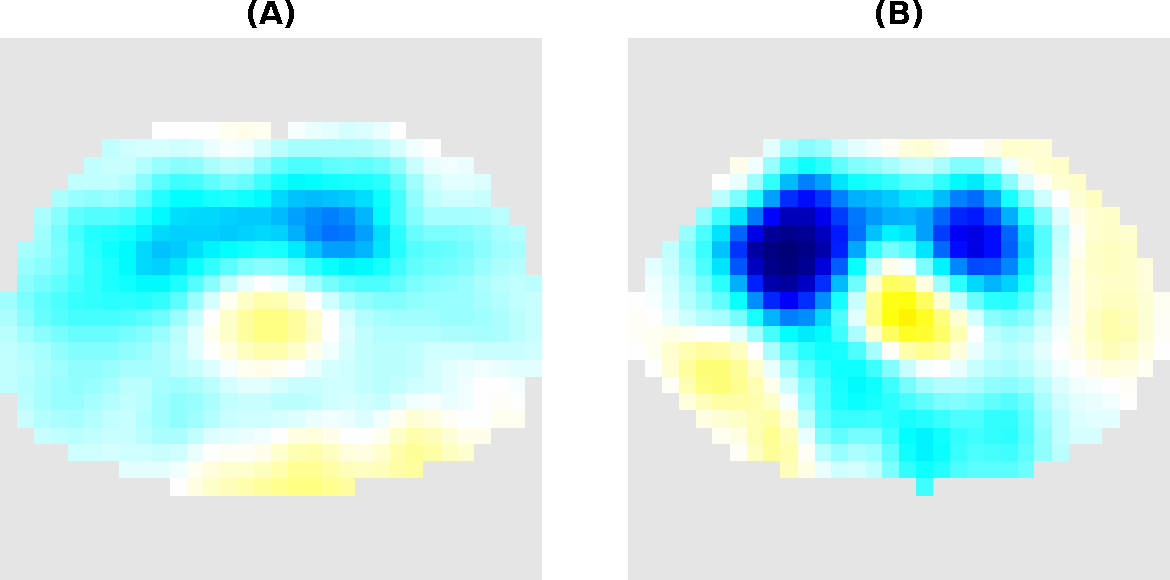
\includegraphics[width=\textwidth]{chapter5-CT_to_mesh/imgs/basic_vs_advanced_3_cropped.pdf}
\caption{\label{fig:ct_mesh_breath}%
Single breath using: A) generic model B) custom model
}
\end{figure}

Results in figure~\fref{fig:breath} show a reconstructed image 
with more separable lungs in the enhanced model, and a mean GI index for each breath in the 
1 minute 
recording that follows 
trend of the ventilated lung percentage in table~\ref{tbl:twocol}.

\begin{table}
  \centering
  \caption{\label{tbl:twocol} %
  Ventilated lung estimate vs. GI index scores.}
  \begin{tabular}{|p{1.2cm}|p{1.5cm}|p{1.8cm}|p{1.7cm}|}
    \hline
  Subject & Ventilated lung (\%) &
  GI (basic model) & GI (custom model) \\ \hline
  1 & 99.9 & 0.353\pm0.004& 0.690\pm0.005 \\ 
  2 & 85.5 & 0.640\pm0.022& 0.771\pm0.020  \\
  3 & 79.6 & 0.695\pm0.007& 0.857\pm0.009  \\
  4 & 27.0 & 0.614\pm0.011& 1.81\pm0.053 \\\hline
  \end{tabular}
  \vspace{-1em} 
\end{table}


\begin{figure}
\centering
% Use the following line with your images (pdf preferred)
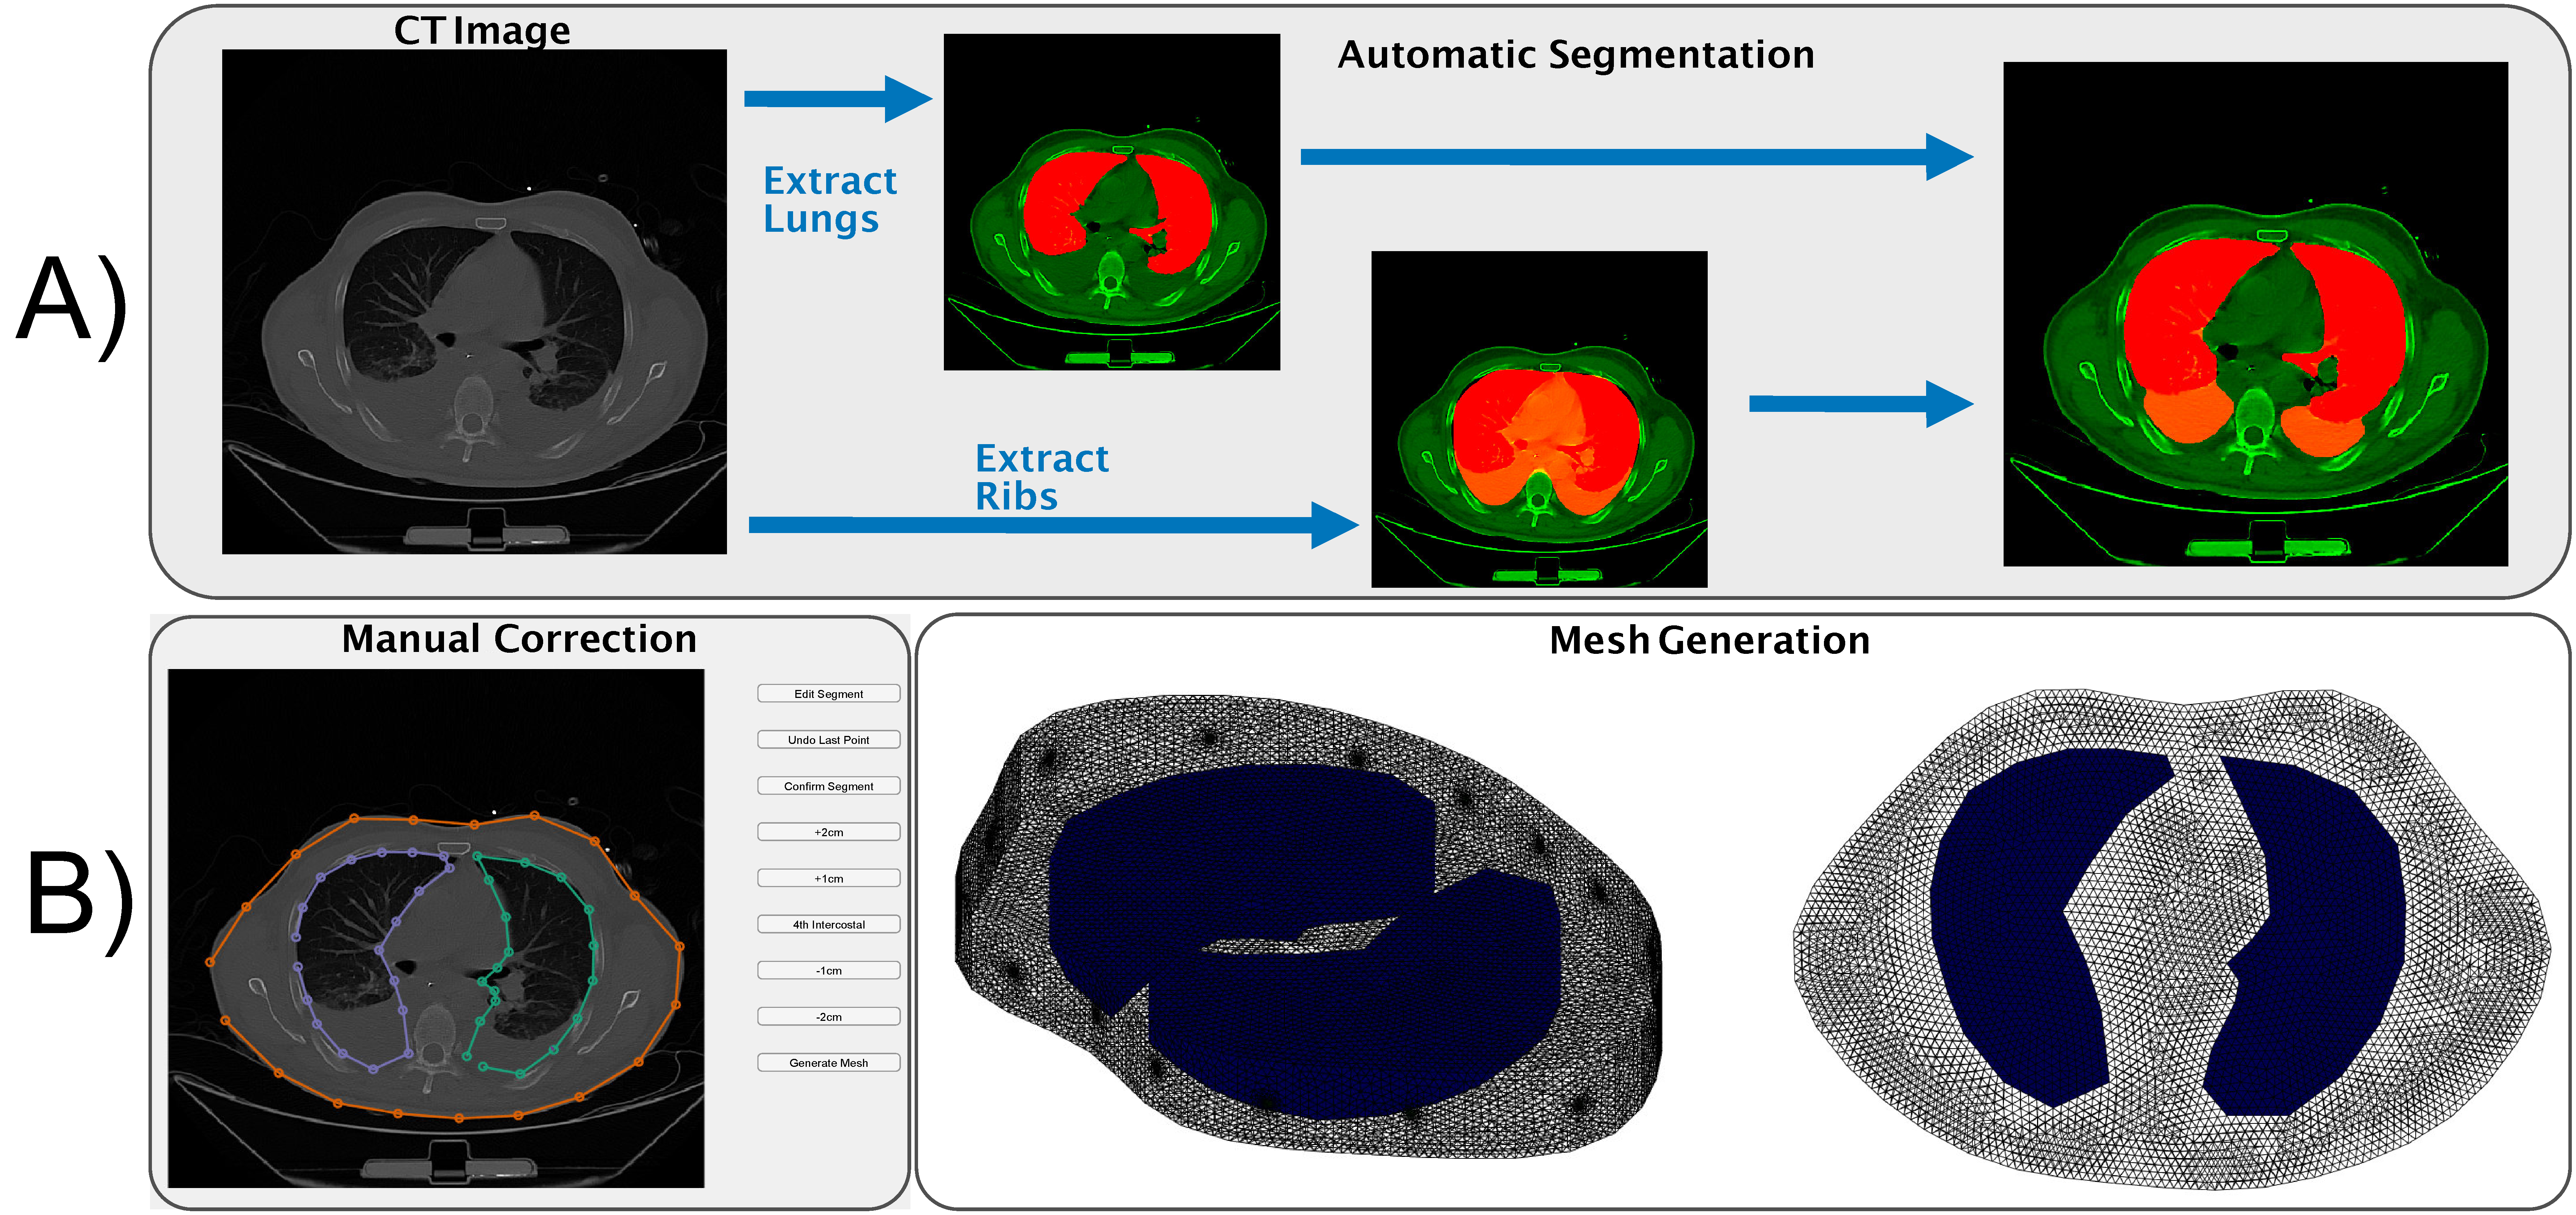
\includegraphics[width=\textwidth]{chapter5-CT_to_mesh/imgs/methods_figure.pdf}
\caption{\label{fig:segment_overview}%
An overview of the segmentation and editing process showing: 
A) A sample raw CT which was thresholded, scaled and adjusted over several 
adjacent slices to identify
the lung regions and an enclosed rib area, and the resulting lung estimate; and
B) A screen  capture of the manual mesh correction process and 2 views of the generated
mesh.
}
\end{figure}